\chapter{Le interfacce utente}

Un'interfaccia è qualcosa che sta fra due facce. E' il punto di contatto fra due sistemi che tentano di comunicare. L'interfaccia serve quindi per comunicare. Un'interfaccia può essere fisica (pulsanti), grafica (immagini a monitor) o di altre forme come per esempio un interprete, un traduttore simultaneo o un mediatore culturale. 

Le interfacce possono far comunicare due macchine fra loro come nel caso del processore che tramite l'interfaccia USB scambia dati con la stampante. Oppure possono far comunicare l’uomo con la macchina, come il cruscotto di un’auto, i cursori di un amplificatore, il rubinetto del lavandino, il manubrio e i pedali della bicicletta.

Un'interfaccia utente è quindi sempre composta da due parti. Una di queste parti appartiene ad una persona l'altra ad uno strumento. Lo strumento è ciò che compie l'azione, l’interfaccia è ciò che serve per permettere all'utente di guidare lo strumento nell'esecuzione dell'azione. Per esempio, in un coltello la lama è lo strumento (che compie l'azione del tagliare), il manico è l’interfaccia che consente all'uomo di usare la lama senza tagliarsi e quindi di guidare lo strumento in maniera soddisfacente. 

\begin{figure}[!h]
	\centering
	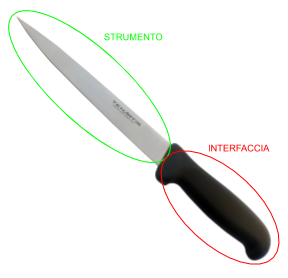
\includegraphics[width=0.7\textwidth]{immagini/interfaccia.png}
	\caption{L'interfaccia è ciò che consente l'interazione, il controllo e la comunicazione con uno strumento.}
\end{figure}


Quando parliamo di \textbf{User Interface o UI}, in italiano Interfaccia Utente, parliamo quindi dello spazio di un sistema dove avviene l'interazione fra uomo-macchina. Tipicamente, si parla di UI in ambito informatico e tecnologico e quindi le interfacce utente sono comunemente identificate come sistemi atti a mettere in comunicazione l'uomo con computer, sistemi informatici e oggetti intelligenti.

L'obiettivo primario dell'interazione fra uomo e macchina è quello di consentire all'utente di controllare e far funzionare la macchina in modo efficace. L'interfaccia deve quindi essere progettata per semplificare l'interazione fra l'uomo e la macchina rendendo così l'esperienza d'uso piacevole e prolifica. L'interazione fra uomo e macchina deve sempre essere facile, efficiente e divertente così da massimizzare la User Experience del prodotto.

E' importante ricordare che l'uomo si è evoluto grazie alla sua capacità di adattamento che ha la sua massima espressione nel libero arbitrio e nella capacità di prendere decisioni non necessariamente basate sulla logica ma piuttosto sulle sensazioni e intuizioni. Viceversa le macchine hanno un comportamento puramente deterministico e pertanto non hanno nessuna capacità di adattamento. L'interfacci uomo macchina va quindi ad avere un ruolo fondamentale nell'interazione fra le parti dal momento che abilita la comunicazione fra due realtà aventi principi e modalità di "funzionamento" diametralmente opposte.

Un'interfaccia ben progettata consente all'utente di controllare l'apparato richiedendo uno sforzo fisico e cognitivo minimo. La buona interfaccia massimizza inoltre la quantità di informazioni utili trasferite all'utente durante l'interazione evitando un sovraccarico informativo che provocherebbe nell'utente confusione e quindi frustrazione.

\begin{figure}[!h]
	\centering
	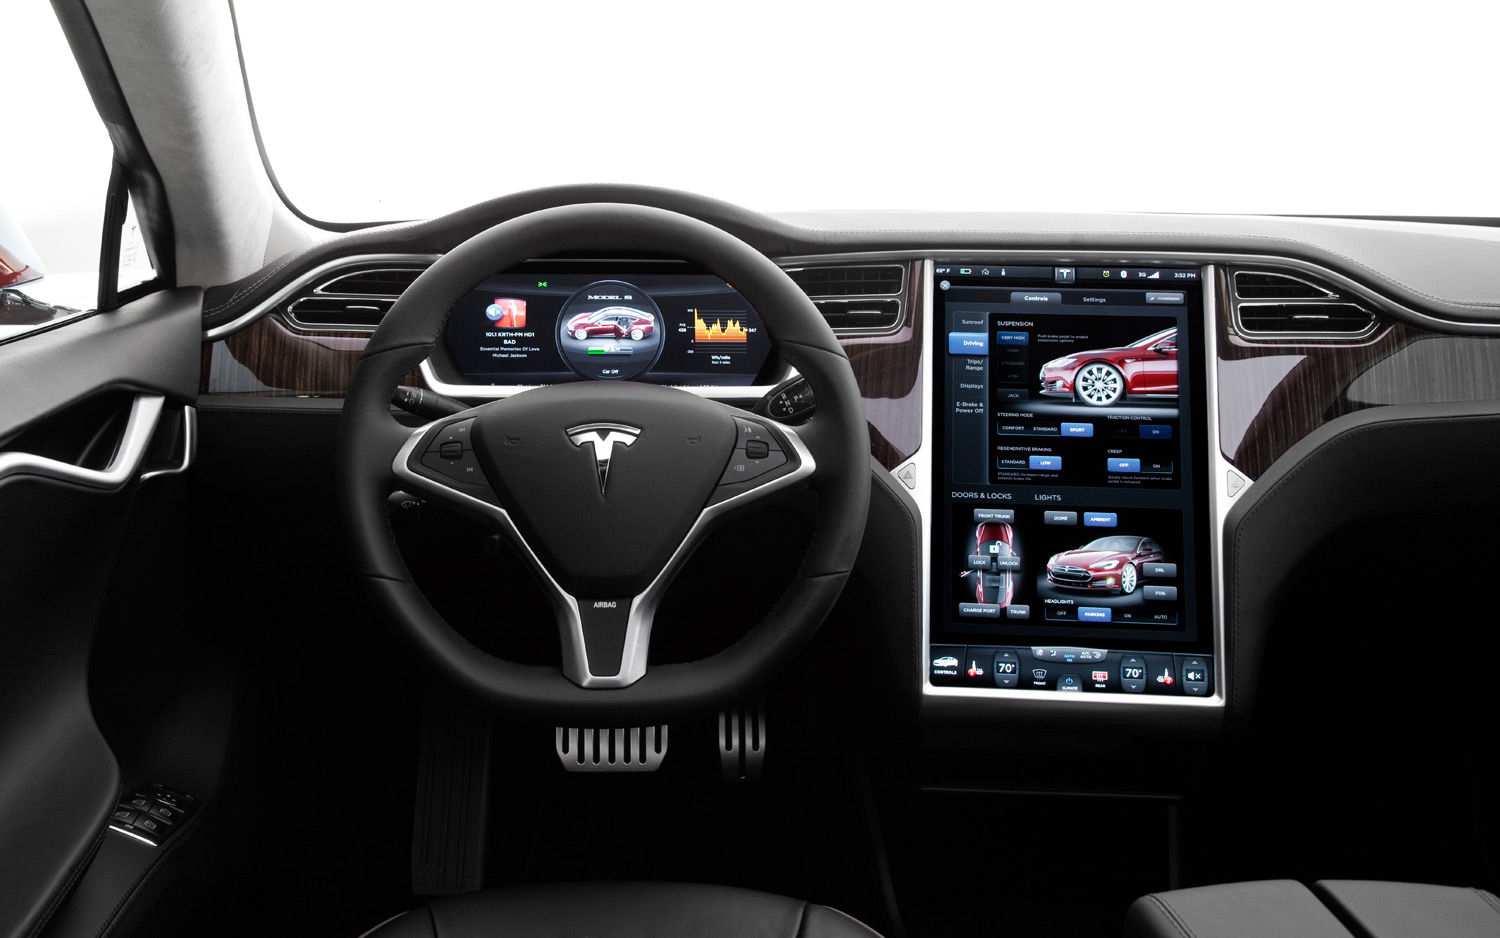
\includegraphics[width=0.9\textwidth]{immagini/tesla.jpg}
	\caption{Cruscotto della Tesla model S. Fonte: 
https://pinxcars.com/2013-tesla-model-s-cockpit/}
\end{figure}

Per questo motivo, la progettazione di un'interfaccia è per definizione un'attività interdisciplinare che va oltre la programmazione grafica e abbraccia la psicologia, le neuroscienze, il design e la fisica.

Le interfacce sono organizzabili secondo livelli. L' \textbf{HID o Human Interface Device} è la periferica grazie al quale l'utente interagisce con il sistema; come ad esempio mouse, monitor, gamepad, ecc.. Lo \textbf{HMI o Human Machine Interface} è invece un concetto che astrae dall' HID. Con HMI, si intende infatti, tutto il sistema di interazione uomo macchina che usa l'HID come elemento di contatto fisico con l'utente. Nel computer per esempio, la HMI è il sistema mouse+cursore+finestre. Il mouse e il monitor sono HID.

Quando la macchina in questione è un computer, HMI diviene \textbf{HCI o Human Computer Interface}.

\section{Classificazione delle interfacce}
Le interfacce utente sono tipicamente organizzate sulla base dei sensi che utilizzano per stabilire l'interazione fra umano e macchina. Gli umani possiedono cinque sensi (Tatto, Vista, Udito, Olfatto e Gusto). Questo porta ad identificare cinque categorie di interfacce possibili, più una sesta che è legata al cosidetto senso dell'orientamento (balance in inglese) che però non è considerato un senso vero e proprio nella fisiologia umana.

Possiamo quindi organizzare le interfacce in 6 categorie:
\begin{itemize}
	\item \textbf{Tactile UI} (touch, tatto)
	\item \textbf{Visual UI} (sight, vista)
	\item \textbf{Auditory UI} (sound, udito)
	\item \textbf{Olfactory UI} (smell, olfatto)
	\item \textbf{Gustatory UI} (taste, gusto)
	\item \textbf{equilibrial UI} (balance, equilibrio)
\end{itemize}

La maggior parte delle interfacce utente utilizza però più di un senso umano per stabilire il collegamento. Le interfacce che usano più di un senso sono dette \textbf{CUI o Composite User Interface}.
Le più comuni e note CUI sono chiaramente le famose \textbf{GUI o Graphical User Interface}, le quali sono composte da interfacce grafiche (visual) e tattili (tactile). 

Se ad una GUI andiamo ad aggiungere anche il suono otteniamo una \textbf{MUI o Multimedia User Interface}.

Quindi quando ci si riferisce all'interfaccia di una app con il termine GUI spesso compiamo un errore perchè ormai la maggior parte dei dispositivi informatici ha anche una sorgente sonora che è utilizzata durante l'interazione (feedback audio del touch sullo schermo, per esempio) e quindi ci troviamo di fronte ad una MUI e non ad una GUI.


È bene sottolineare che \textbf{estendere le interfacce con più canali (sensi) non è sempre una buona idea
}. Prendiamo ad esempio i video di Facebook, i video vengono riprodotti di default con l'audio disattivato per aumentare l'usabilità del sistema. Gli ingegneri di Facebook si sono accorti infatti che la maggioranza delle persone che visualizzando i video, mutavano immediatamente il suono per varie ragioni (e.g. privacy o utilizzo di Facebook in momenti non opportuni), quindi hanno reso questa opzione di default. Ovviamente se ragionassimo in termini di capacità e possibilità dell'interfaccia sembrerebbe assurdo bloccare di default l'utilizzo di un canale.
Questo processo di anali ha portato poi a far evolvere il mondo dei video online inserendo di default i sottotitoli. Siamo quindi in una situazione in cui per aumentare l'usabilità del sistema se ne riducono le funzionalità (di default).

%Questo, oltre ad essere un ottimo esempio di MUI riprogettata in GUI, è anche un esempio di tecnica ideata per gli utenti disabili e riusata per far fruire il prodotto a quelle personas che lo utilizzano in momenti in cui non possono usufruire dell'audio.

\begin{figure}[!h]
	\centering
	
\includegraphics[width=0.9\textwidth]{immagini/flora_video.png}
	\caption{I video di Facebook sono in muto di default per aumentare l'usabilità del sistema. Fonte: 
https://www.facebook.com/Lastknight/posts/10158944882367053}
\end{figure}



\section{Categorizzare le CUI}
Le CUI possono essere categorizzare in tre diverse macrocategorie:

\begin{itemize}
	\item \textbf{Standard}: usano dispositivi standard come tastiere, mouse e monitor
	\item \textbf{Virtual}: Bloccano all'utente l'interazione con il mondo reale e creano un mondo virtuale che funge da interfaccia fra l'utente e la macchina.
	\item \textbf{Augmented}: Non bloccano all'utente la percezione del mondo reale ma la vanno ad arricchire. L'interfaccia è quindi un mix di contenuti reali e virtuali che vanno ad arricchire la realtà \textbf{espandendola}.
\end{itemize}

\begin{figure}[!h]
	\centering
	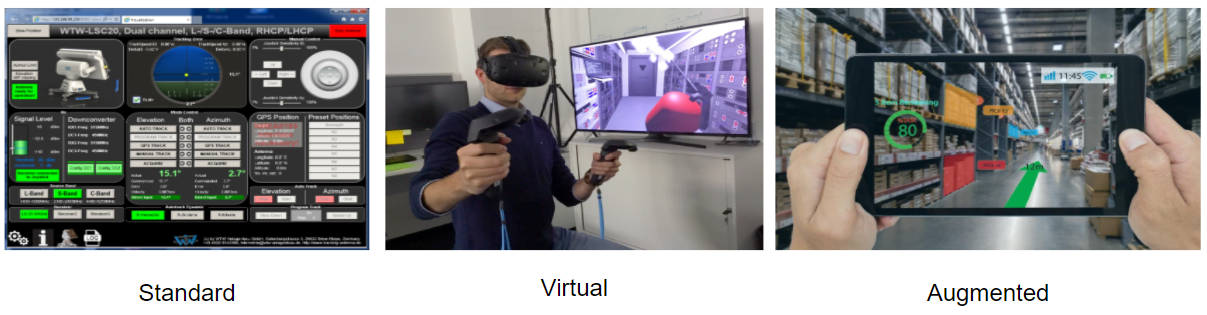
\includegraphics[width=\textwidth]{immagini/standard-virtual-interfaces.png}
	\caption{Le interfacce possono essere di tipo Standard, Virtuale o Aumentato.}
\end{figure}

Le CUI possono essere anche \textbf{classificate tramite il numero di sensi che utilizzano}. Ad esempio, lo \textit{Smell-O-Vision} è una CUI standard 3S, cioè è una normale interfaccia di tipo standard che nell'utilizzo coinvolge 3 sensi dell'utente (Visione, Udito e Olfatto). Se si aggiungesse un quarto senso (per esempio le poltrone mobili dei cinema 4D) diventerebbe 4S.

Quando un'interfaccia utente interagisce con tutti i sensi umani viene chiamata \textbf{Qualia Interface}. il termine Qualia interface deriva dalla \textbf{teoria filosofica dei Qualia} (https://it.wikipedia.org/wiki/Qualia).

Il Microsoft Reactable è un interessante esempio di interfaccia aumentata 3S (MUI) (Figura \ref{fig:react-table}).

\begin{figure}[!h]
	\centering
	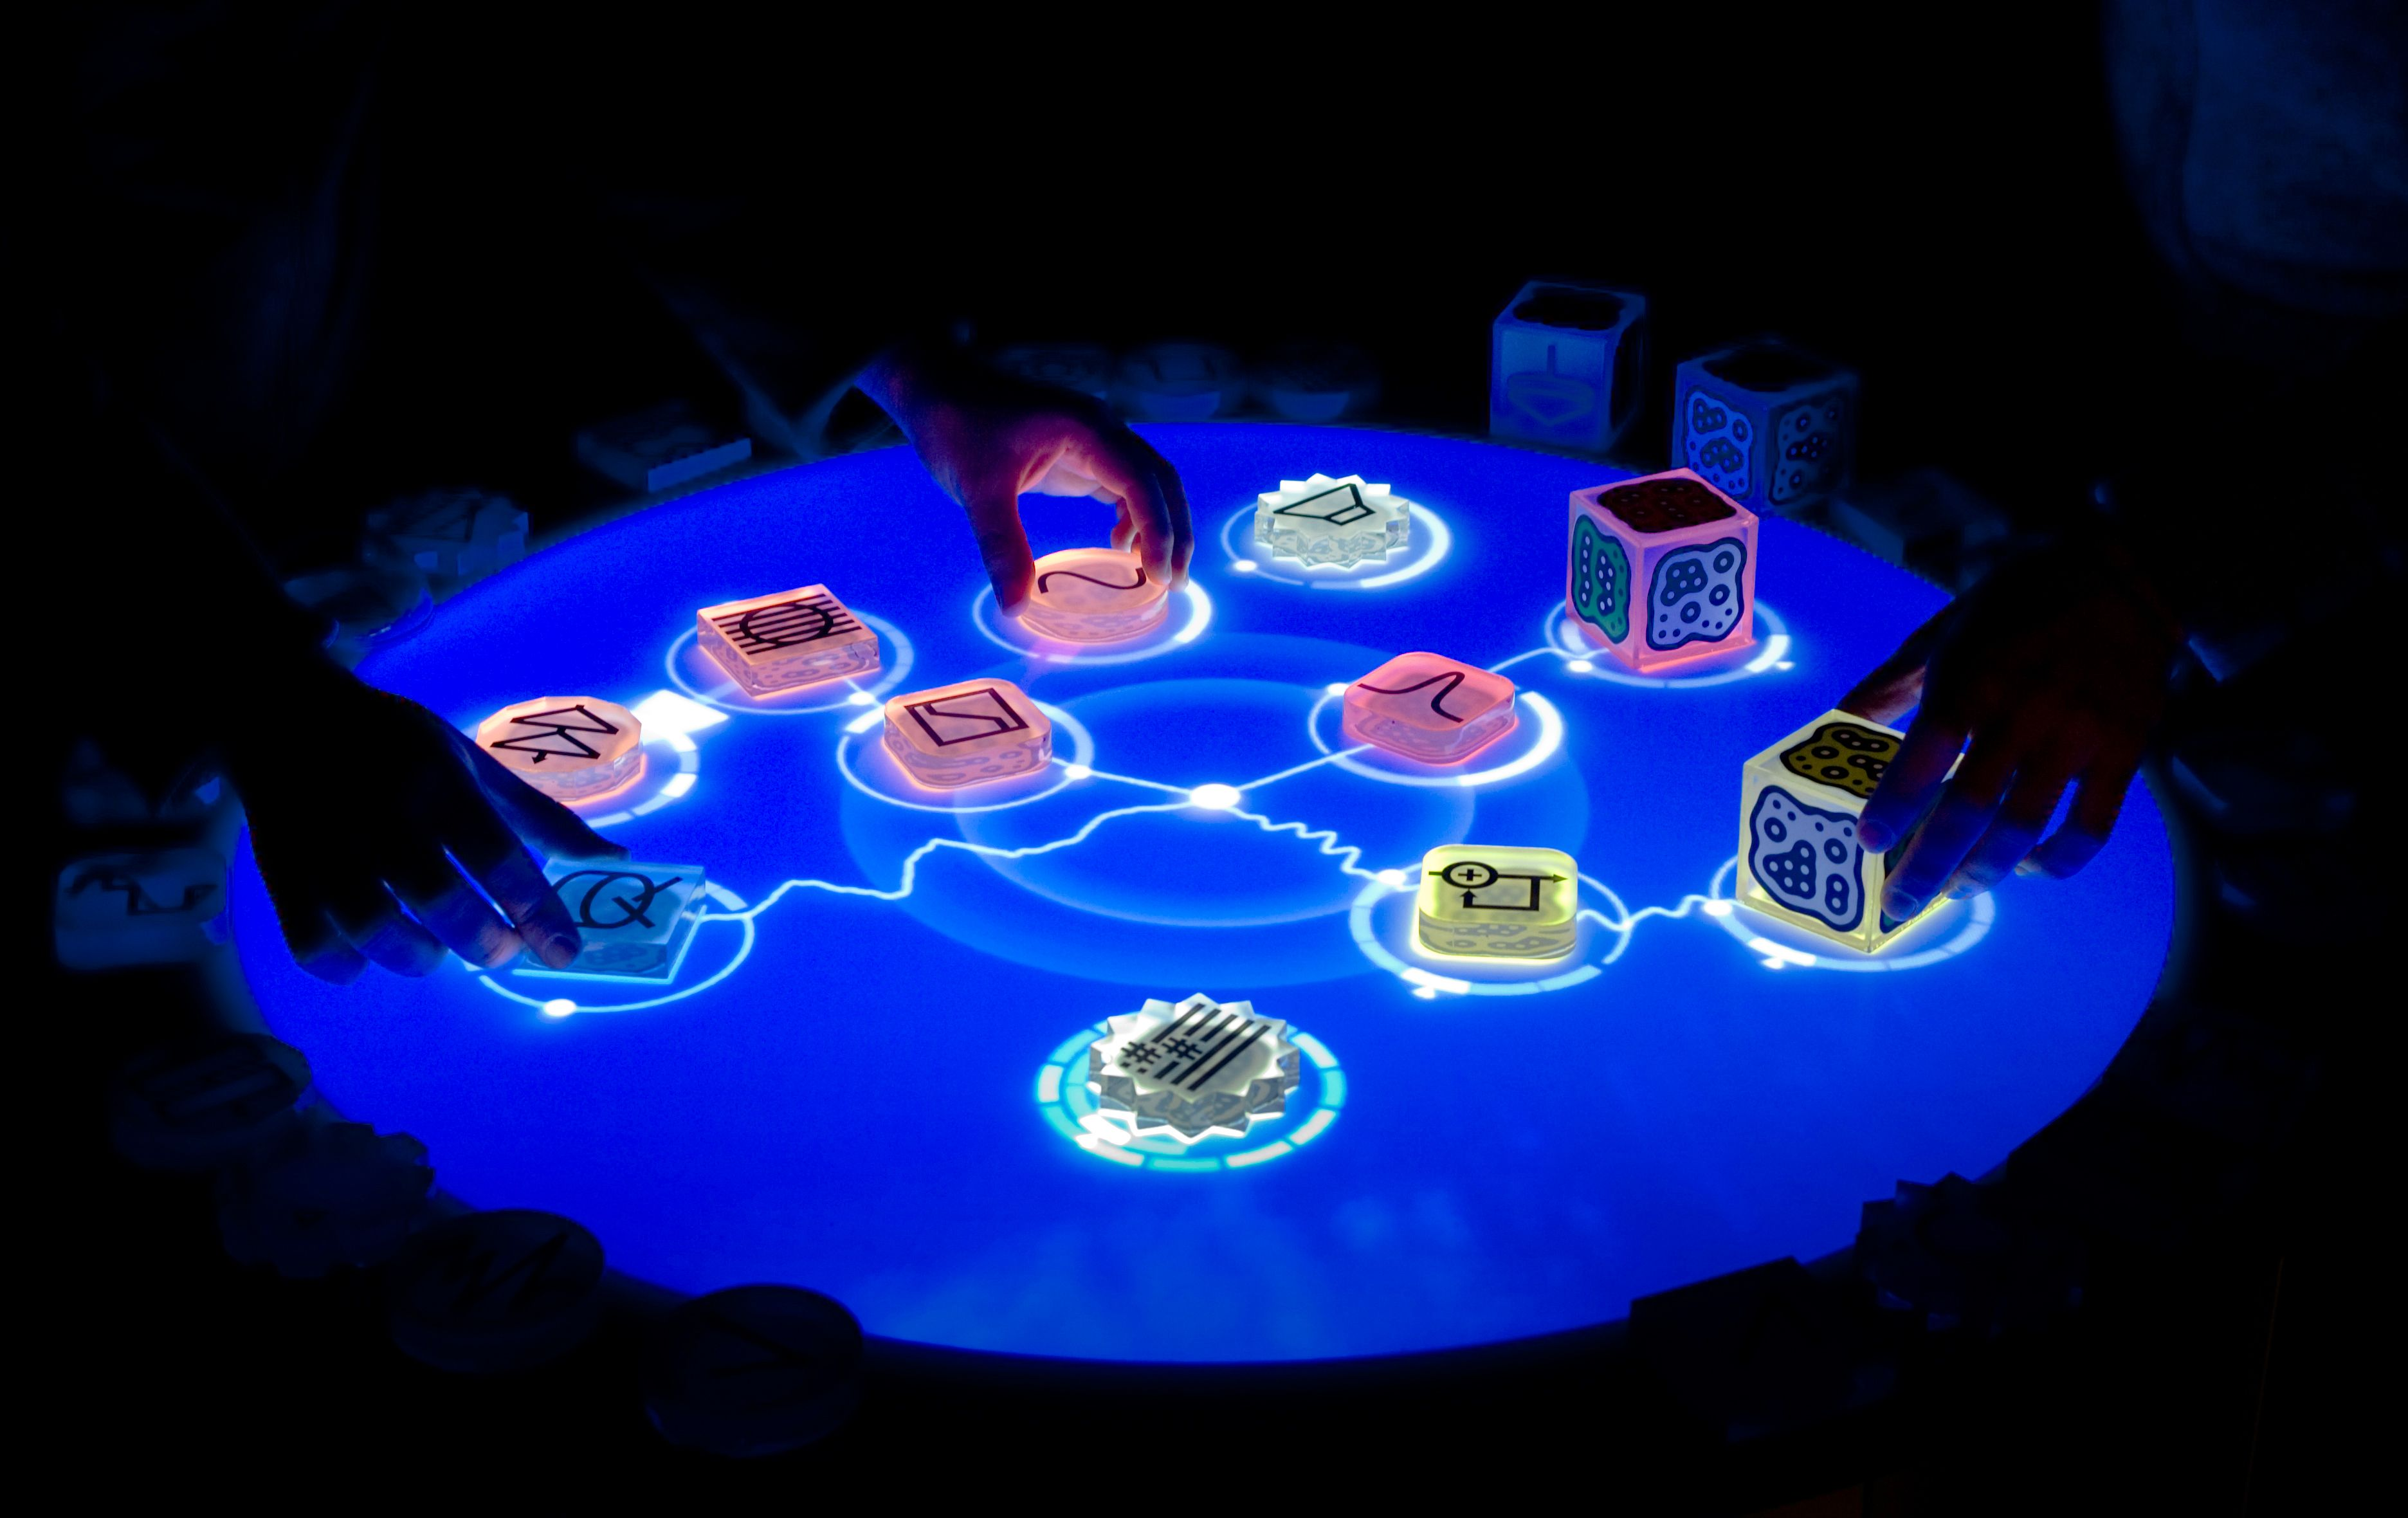
\includegraphics[width=\textwidth]{immagini/react.jpg}
	\caption{Microsoft Reactable.}
	\label{fig:react-table}
\end{figure}



\pagebreak

